\documentclass[10pt,a4paper]{article}

\usepackage[T1]{fontenc}
\usepackage{lmodern}
\usepackage[a4paper,margin=15mm]{geometry}
\usepackage{microtype}
\usepackage{booktabs}
\usepackage{tabularx}
\usepackage[table]{xcolor}
\usepackage[hidelinks]{hyperref}
\usepackage{titlesec}
\usepackage{enumitem}
\usepackage{tikz}
\usetikzlibrary{arrows.meta,backgrounds,fit,positioning}

\definecolor{ink}{HTML}{172033}
\definecolor{teal}{HTML}{087E76}
\definecolor{blue}{HTML}{3157C8}
\definecolor{canvas}{HTML}{EEF2F3}
\definecolor{amber}{HTML}{A65D00}
\definecolor{line}{HTML}{AAB5BC}

\hypersetup{
  colorlinks=true,
  urlcolor=blue,
  linkcolor=ink,
  pdftitle={TailorCV: A Cloud-Based Resume Tailoring Platform},
  pdfauthor={Khang Vuong}
}

\setlength{\parindent}{0pt}
\setlength{\parskip}{3.2pt}
\setlength{\tabcolsep}{5pt}
\renewcommand{\arraystretch}{1.05}
\pagestyle{plain}
\raggedbottom

\titleformat{\section}
  {\large\bfseries\color{ink}}
  {}{0pt}{}
\titlespacing*{\section}{0pt}{7pt}{2pt}
\titleformat{\subsection}
  {\normalsize\bfseries\color{teal}}
  {}{0pt}{}
\titlespacing*{\subsection}{0pt}{5pt}{1pt}

\begin{document}

\begin{center}
  {\LARGE\bfseries\color{ink} TailorCV: A Cloud-Based Resume Tailoring Platform}\\[-1pt]
  {\small Khang Vuong \quad|\quad 49064010 \quad|\quad INFS3208 Cloud Computing}
\end{center}

\section{Introduction}

\subsection{Background and motivation}
TailorCV is a web application that converts a text-based PDF resume into a consistent, job-targeted resume. Applicants frequently adapt the same resume for different roles, but manually identifying relevant evidence, reorganising content, and recreating a readable PDF is repetitive and error-prone. General-purpose generative AI can accelerate this work, yet unconstrained generation may invent skills, employers, dates, or achievements. TailorCV addresses this problem through a structured workflow that retains the source resume and validates AI selections against it.

\subsection{Objective and features}
The objective is to provide a responsive, end-to-end resume-tailoring workflow without requiring an account. The implemented MVP provides six user-facing functions: PDF upload and validation; structured extraction and confirmation; job-description storage; evidence-grounded AI tailoring; HTML preview with change and missing-requirement summaries; and ATS-friendly PDF download. It accepts selectable-text PDFs up to 5 MB and persists resumes, jobs, and tailoring runs. Tailored output requires user review and is not presented as a guaranteed ATS score.

\subsection{Traditional limitations and cloud benefits}
A desktop-only implementation ties processing and stored data to one machine, complicates updates, and cannot share capacity when demand changes. A single server also couples the user interface, document processing, AI integration, and database failure domains. Manual deployment creates downtime and inconsistent environments.

Containerised cloud services instead separate the public workflow from AI processing and persistence. Kubernetes can maintain replicas, replace failed Pods, distribute requests through Services, and perform rolling updates with rollback. Readiness probes keep unready Pods out of Service endpoints, while persistent storage separates database data from container lifetimes. ConfigMaps and Secrets keep deployment settings and credentials out of images. These capabilities improve scalability and resilience, but do not guarantee zero downtime or improve AI correctness.

\section{Technical solution}
The React 19 and TypeScript frontend is built with Vite. Nginx serves the built React app and reverse-proxies \texttt{/api/v1/*} requests to the internal Java 21 Spring Boot \texttt{resume-service}. Java validates PDFs, extracts text with PDFBox, owns the public REST API, persists data through Spring Data JPA and Flyway, and produces matching HTML/PDF output with Thymeleaf and OpenHTMLtoPDF. PostgreSQL 17 stores bounded original PDF bytes, extracted text, canonical JSON, job descriptions, and tailoring runs.

The stateless Python 3.12 FastAPI \texttt{ai-service} owns strict Pydantic parsing and tailoring contracts. Default extraction is conservative and rule-based. Optional OpenAI structured output uses bounded timeouts and schema validation. Tailoring selects source skills and experience bullets by index; Python then reconstructs the result from source data to reject unsupported claims. Provider failures are exposed only as sanitised errors. Docker Compose supports local development; the same services are containerised for GKE.

\newpage

\section{Cloud deployment and cost}
The GKE deployment uses a two-node, zonal Standard cluster in Sydney. Separate Deployments specify one frontend Pod, two Java Pods, and two Python Pods. A public HTTP LoadBalancer Service exposes only the frontend; Java, Python, and PostgreSQL use private ClusterIP Services. Kubernetes probes, resource requests/limits, a ConfigMap, and a Secret control operation. PostgreSQL 17 runs as one StatefulSet Pod with a 10 Gi persistent-volume claim. Java Pods prefer different nodes. Backend replicas and Pod replacement improve resilience but cannot guarantee uninterrupted service; the frontend and database remain single points of failure.

\begin{table}[!ht]
  \centering
  \small
  \rowcolors{2}{canvas}{white}
  \begin{tabularx}{\linewidth}{@{}Xl r@{}}
    \toprule
    \textbf{Resource} & \textbf{Planning assumption} & \textbf{USD/month} \\
    \midrule
    GKE management & Calculator: zonal cluster & \$73.00 \\
    Compute Engine & Calculator: 2 \texttt{e2-standard-2} nodes & \$138.82 \\
    Node boot disks & Calculator: 60 GiB balanced PD & \$8.10 \\
    Conditional GKE credit & If available on the billing account & $-\$73.00$ \\
    Other infrastructure & Provisional: L4 LB, network, PVC, images & $\sim\$29$ \\
    Build and AI & Free-tier builds, demo model usage & $<\$1$ \\
    \midrule
    \textbf{Estimated total} & \textbf{Assuming credit; before tax} & \textbf{\$176--177} \\
    \bottomrule
  \end{tabularx}
\end{table}

\noindent\fcolorbox{amber}{white}{%
  \parbox{0.965\linewidth}{\small Google Calculator CSV (20 Oct 2026): \$219.92 for cluster, nodes, and boot disks before credit. The credit is conditional; other items are separate estimates. Without credit, the planning total is \$249--250/month. Actual billing may differ.}}

\section{Architecture design}

\begin{figure}[!ht]
\centering
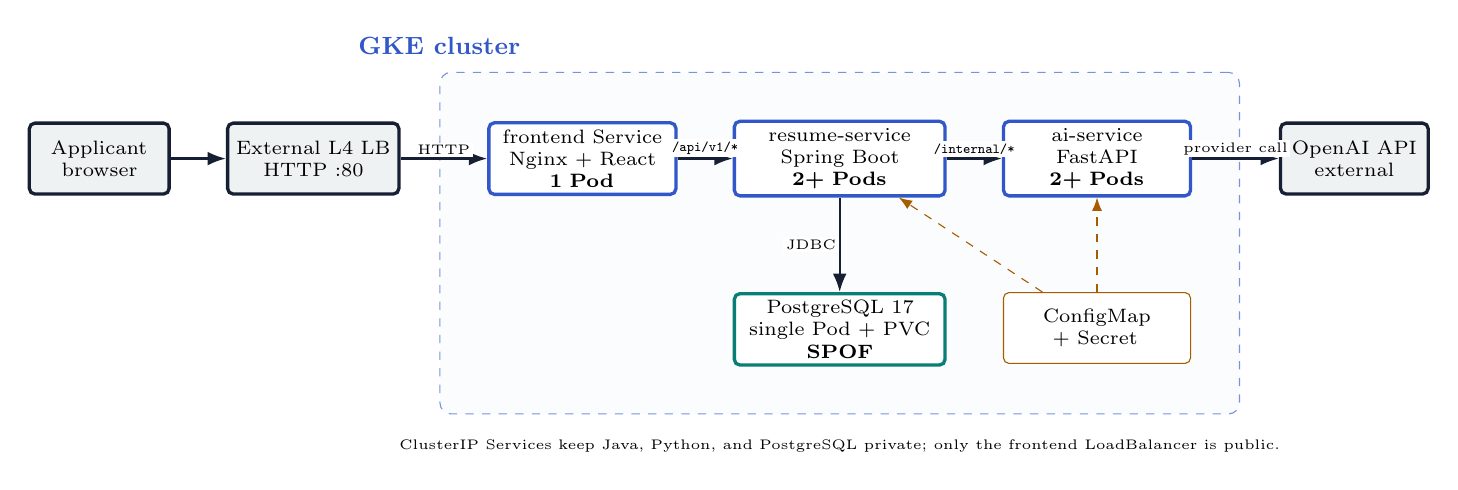
\begin{tikzpicture}[
  font=\scriptsize,
  >=Latex,
  flow/.style={-Latex,thick,draw=ink},
  support/.style={-Latex,dashed,draw=amber},
  box/.style={draw=line,rounded corners=2pt,fill=white,align=center,
              minimum height=9mm,text width=22mm,inner sep=2.5pt},
  service/.style={box,draw=blue,very thick},
  data/.style={box,draw=teal,very thick},
  external/.style={box,draw=ink,very thick,fill=canvas},
  label/.style={font=\tiny,align=center,fill=white,inner sep=1pt}
]
  \node[external,text width=16mm] (browser) {Applicant\\browser};
  \node[external,right=7mm of browser,text width=20mm] (lb) {External L4 LB\\HTTP :80};

  \node[service,right=11mm of lb] (front) {frontend Service\\Nginx + React\\\textbf{1 Pod}};
  \node[service,right=7mm of front,text width=25mm] (resume) {resume-service\\Spring Boot\\\textbf{2+ Pods}};
  \node[service,right=7mm of resume] (ai) {ai-service\\FastAPI\\\textbf{2+ Pods}};
  \node[external,right=11mm of ai,text width=17mm] (openai) {OpenAI API\\external};

  \node[data,below=12mm of resume,text width=25mm] (db) {PostgreSQL 17\\single Pod + PVC\\\textbf{SPOF}};
  \node[box,draw=amber,below=12mm of ai,text width=22mm] (config) {ConfigMap\\+ Secret};

  \begin{scope}[on background layer]
    \node[draw=blue!65,dashed,rounded corners=4pt,fill=blue!2,
          fit=(front)(resume)(ai)(db)(config),inner sep=6mm] (cluster) {};
  \end{scope}

  \draw[flow] (browser) -- (lb);
  \draw[flow] (lb) -- node[label,above]{HTTP} (front);
  \draw[flow] (front) -- node[label,above]{\texttt{/api/v1/*}} (resume);
  \draw[flow] (resume) -- node[label,above]{\texttt{/internal/*}} (ai);
  \draw[flow] (ai) -- node[label,above]{provider call} (openai);
  \draw[flow] (resume) -- node[label,left]{JDBC} (db);
  \draw[support] (config) -- (resume);
  \draw[support] (config) -- (ai);

  \node[font=\small\bfseries\color{blue},anchor=south west,
        above=1mm of cluster.north west] {GKE cluster};
  \node[font=\tiny,align=center,below=2mm of cluster.south] {ClusterIP Services keep Java, Python, and PostgreSQL private; only the frontend LoadBalancer is public.};
\end{tikzpicture}
\caption{GKE deployment topology: only the frontend is publicly reachable.}
\end{figure}

The browser never calls Python or PostgreSQL directly. Java orchestrates upload, persistence, tailoring, and export, while Python remains stateless and independently scalable. Demo commands exercise scaling, Service routing, Pod replacement, rolling update, and rollback. Current limitations include no authentication, HTTPS, or OCR; dependence on an external model; one frontend Pod; and non-replicated PostgreSQL. Only fictional applicant data should be used.

\end{document}
